\documentclass{article}
\usepackage{graphicx}
\usepackage[margin=1.5cm]{geometry}
\usepackage{amsmath}
\usepackage{url}

\begin{document}

\title{PhET and Lab Activity: Unit 1, Acceleration and Kinematics}
\author{Prof. Jordan C. Hanson}

\maketitle

\section{Position, Velocity, and Acceleration}

\begin{enumerate}
\item Open the following link and scroll to the bottom of the page: \url{https://openstax.org/books/college-physics/pages/2-4-acceleration}.  
\item Open the PhET simulation.  Click on the link for the Moving Man Simulation, entitled \textbf{Click to View Content.}
\item The introduction tab at the top left will help you learn the controls.  Using the mouse, you can drag the man left and right in one dimension.  His position, velocity, and acceleration will be indicated by the blue, red, and green markers, respectively.
\item Now click on the tab at the top left entitled \textbf{Charts.}
\item Slowly drag the man to the right \textit{at a steady pace.}  Do you observe the following?
\begin{itemize}
\item A linearly increasing position?
\item A (roughly) constant velocity?
\item An acceleration that is basically zero?
\end{itemize}
\item Hit reset at the bottom right, and redo the experiment.  This time, move the man all the way to the right, then move him all the way to the left.  As accurately as you can, with labeled axes and units, draw his position below: \\ \vspace{2.0cm}
\item From the position versus time graph you've created, identify the region of positive velocity by looking at the slope.  Calculate the average velocity from the slope of your graph.  Repeat this exercise for the region of negative velocity.  When does acceleration deviate from zero?
\end{enumerate}

\begin{figure}[hb]
\centering
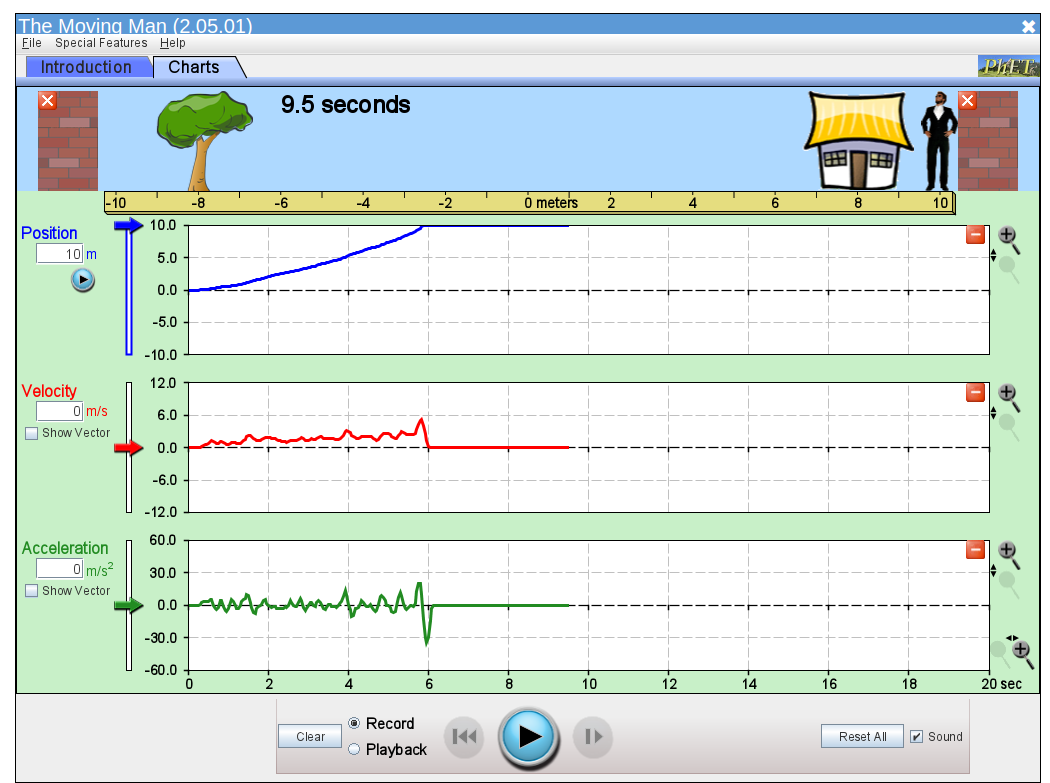
\includegraphics[width=0.4\textwidth]{figures/man.png}
\caption{Example of the PhET simulation.}
\end{figure}

\section{The Acceleration of Gravity, Statistical Mean and Standard Deviation}

This is a simple lab exercise repeating what we did in class with falling marbles.  You will need the stopwatch on your mobile, a small object like a marble, and a ruler or tape measure.  Let's assume we are rolling a marble off the edge of a table.  According to observations of other systems accelerating constantly, when the marble leaves the table the vertical position versus time will be 
\begin{equation}
y(t) = -\frac{1}{2}gt^2 + v_{i,y} t + y_i \label{eq:1}
\end{equation}
In Eq. \ref{eq:1}, $-g$ is the acceleration.  The vector form of acceleration points down, so we give $g$ a minus sign.  The time $t=0$ is when the marble begins to fall, and $v_{i,y}$ is the vertical component of the velocity at $t=0$.  The initial position is $y_i$.  We know that $v_{i,y} = 0$ because we do not \textit{push the marble downwards}, but instead let it fall.  Let the change in height be $h = y(t) - y_i$.  Show that
\begin{equation}
h = -\frac{1}{2}g t^2
\end{equation}
\textbf{This time}, let's solve this equation to solve for $g$.  The result should be
\begin{equation}
g = -\frac{2 h}{t^2}
\end{equation}
\begin{enumerate}
\item Measure $h$ with the ruler, and roll the marble off the table 16 times.  Record 16 measurements of $t$ using a stopwatch.  Use the 16 time values to obtain 16 values for $g$.
\item Let $g_1$ through $g_{16}$ represent your data ($g_i$), and $N = 16$.  Compute the \textit{mean value} of $g$ using the following sum:
\begin{equation}
\bar{g} = \frac{1}{N} \sum_{i=1}^{N} g_i
\end{equation}
Record your results below.
\item Compute the \textit{standard deviation} from the mean value, using the following sum:
\begin{equation}
\sigma_g = \sqrt{\frac{1}{N-1}\sum_{i=1}^{N} (g_i - \bar{g})^2}
\end{equation}
Record your results below.
\item Quote your results like this: $\bar{g} \pm \sigma_g$ in m s$^{-2}$.  Does the accepted average value of 9.81 m s$^{-2}$ fall within the range $[\bar{g} - \sigma_g, \bar{g} + \sigma_g]$?
\end{enumerate}

\end{document}
